%----------------------------------------------------------------------------------------
%	PACKAGES AND OTHER DOCUMENT CONFIGURATIONS
%----------------------------------------------------------------------------------------

\documentclass[fleqn,10pt]{../sty/SelfArx} % Document font size and equations flushed left

%----------------------------------------------------------------------------------------
%	COLUMNS
%----------------------------------------------------------------------------------------

% \setlength{\columnsep}{0.55cm} % Distance between the two columns of text
% \setlength{\fboxrule}{0.75pt} % Width of the border around the abstract

%----------------------------------------------------------------------------------------
%	COLORS
%----------------------------------------------------------------------------------------

\definecolor{color1}{RGB}{0,0,90} % Color of the article title and sections
\definecolor{color2}{RGB}{0,20,20} % Color of the boxes behind the abstract and headings

%----------------------------------------------------------------------------------------
%	HYPERLINKS
%----------------------------------------------------------------------------------------

\usepackage{hyperref} % Required for hyperlinks
\hypersetup{hidelinks,colorlinks,breaklinks=true,urlcolor=color2,citecolor=color1,linkcolor=color1,bookmarksopen=false,pdftitle={Title},pdfauthor={Author}}

%----------------------------------------------------------------------------------------
%	ARTICLE INFORMATION
%----------------------------------------------------------------------------------------

\PaperTitle{HP-12C} % Article title
\JournalInfo{Versão 1.0} % Journal information
\Archive{} % Additional notes (e.g. copyright, DOI, review/research article)

\Authors{Fernando Anselmo} % Authors
\affiliation{} % Author affiliation

\Keywords{HP12C --- Matemática --- Estatística} % Keywords - if you don't want any simply remove all the text between the curly brackets
\newcommand{\keywordname}{Keywords} % Defines the keywords heading name

%----------------------------------------------------------------------------------------
%	ABSTRACT
%----------------------------------------------------------------------------------------

\Abstract{A calculadora da \textit{Hewlett Packard} modelo HP-12C foi lançada em 1981 e se trata de um dos maiores sucessos da empresa, a mais vendida e mais utilizada calculadora do mundo inteiro principalmente na execução de cálculos financeiros e estatísticos. Conheceremos o básico sobre o uso da calculadora que possui mais de 120 funções específicas para uso em negócios e permite trabalhar com 20 diferentes tipos de fluxos de caixa, operações com taxas internas de retorno e valores presentes líquidos.}

%----------------------------------------------------------------------
% Início do Documento
%----------------------------------------------------------------------
\begin{document}
	
\maketitle % mostrar o título
\thispagestyle{fancy} % habilitar o cabeçalho/rodapé das páginas

\section*{Conceitos Básicos}	
A forma de cálculos da HP-12C é pelo sistema RPN (\textit{Reverse Polish Notation}), no qual primeiro se digita o valor, informa sua entrada com a tecla \keystroke{$ENTER$}, digita o segundo valor e a tecla da função desejada. Segue-se esse raciocínio para todas as funções da calculadora, seja com a realização de operações básicas, financeiras ou de estatística; ou seja, primeiro digita-se os valores e por fim a função desejada. 
\begin{figure}[H]
	\centering
	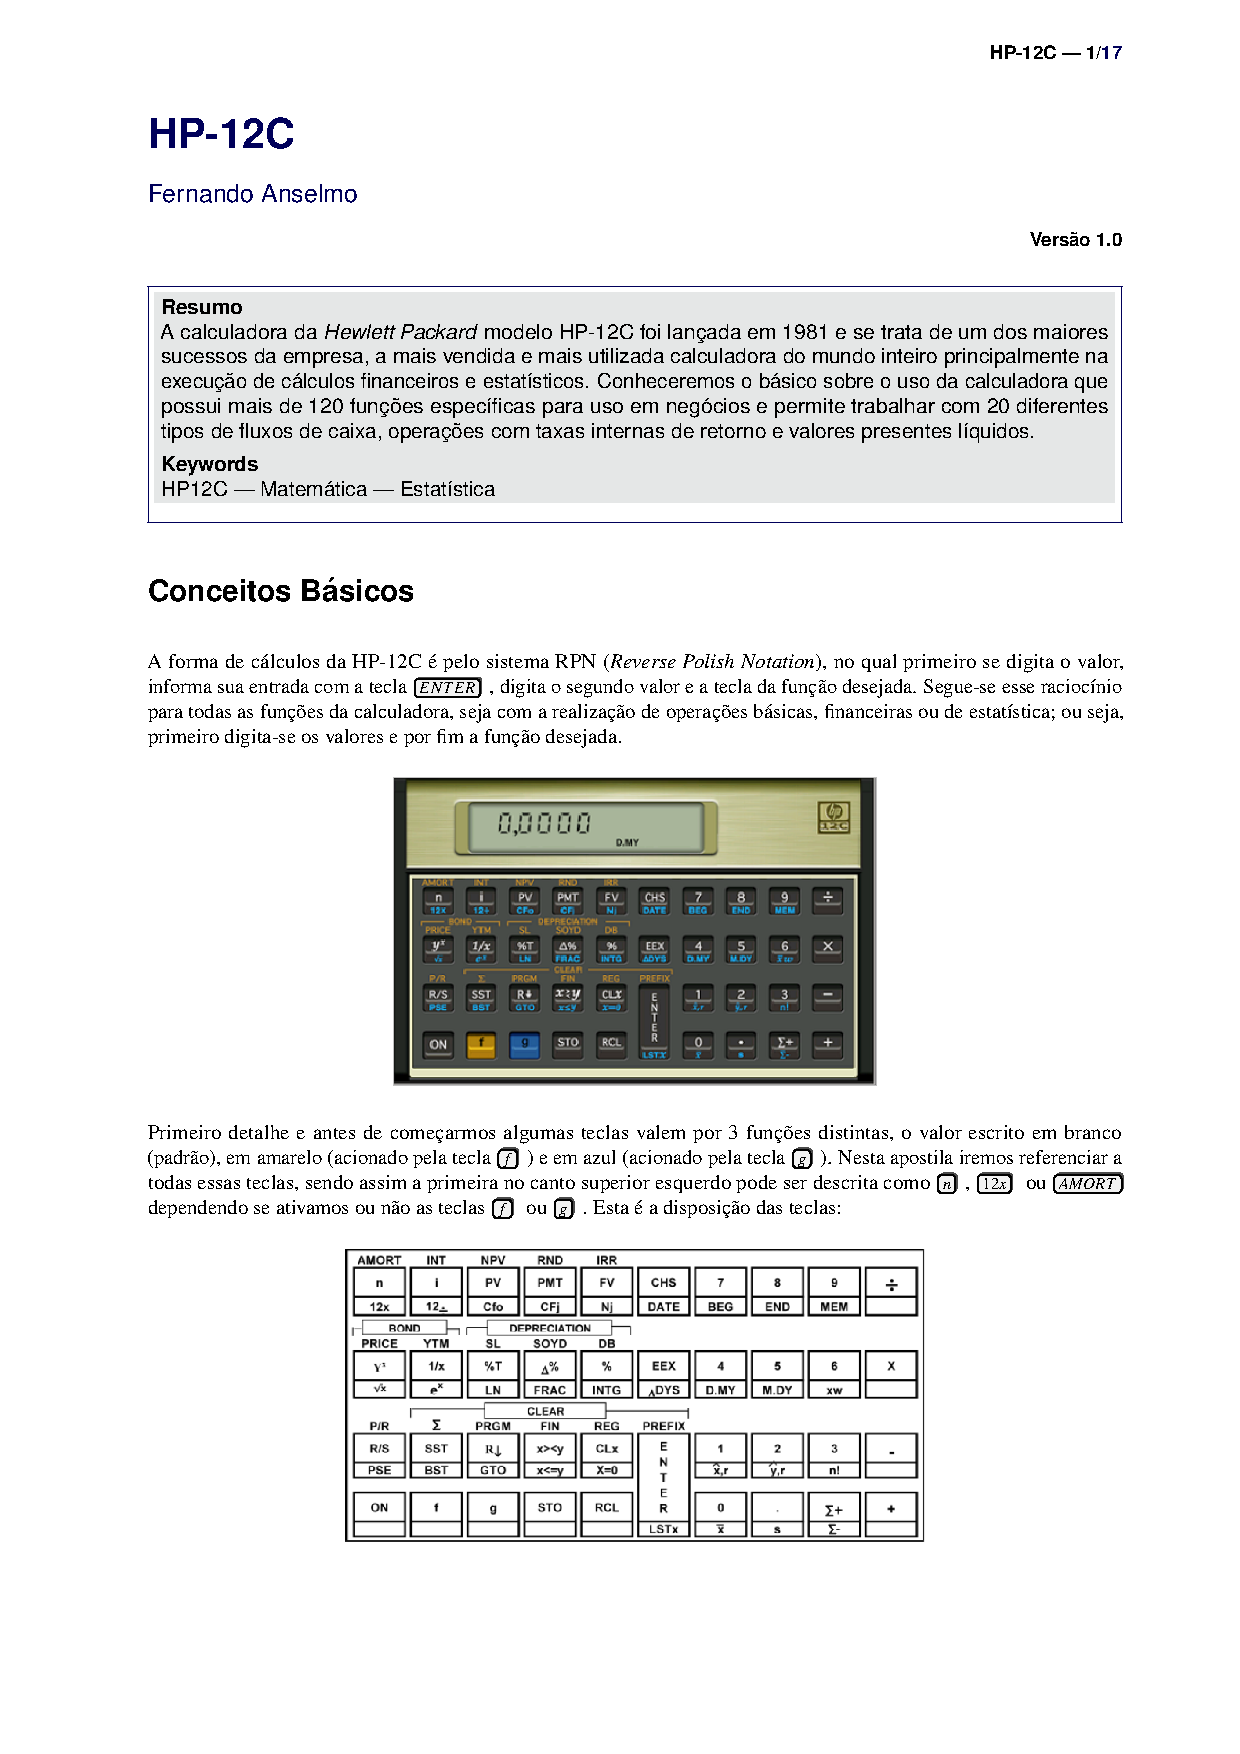
\includegraphics[width=0.5\textwidth]{images/hp12c}
\end{figure}
\vspace{-1em}
Primeiro detalhe e antes de começarmos algumas teclas valem por 3 funções distintas, o valor escrito em branco (padrão), em amarelo (acionado pela tecla \keystroke{$f$}) e em azul (acionado pela tecla \keystroke{$g$}). Nesta apostila iremos referenciar a todas essas teclas, sendo assim a primeira no canto superior esquerdo pode ser descrita como \keystroke{$n$}, \keystroke{$12x$} ou \keystroke{$AMORT$} dependendo se ativamos ou não as teclas \keystroke{$f$} ou \keystroke{$g$}. Esta é a disposição das teclas:
\begin{figure}[H]
	\centering
	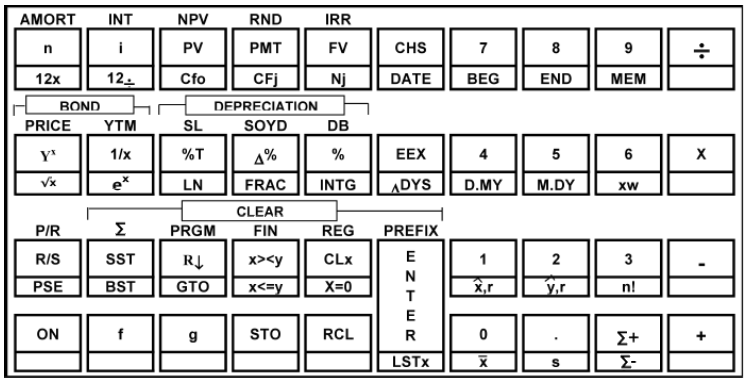
\includegraphics[width=0.6\textwidth]{images/teclado}
\end{figure}

\subsection*{Instalar a Calculadora}
Recomendo fortemente ter a máquina física, porém muitas pessoas possuem receio de comprarem e não se adaptarem, sendo assim podemos baixar uma versão \cite{hp12c} criada com a linguagem Java, testarmos todas as suas potencialidades e decidir.

Basta baixar o arquivo compactado, descompactar que na pasta gerada estão as instruções para seu uso, lembro que e assim como avisa o autor: "\textit{Este software foi desenvolvido para fins educacionais. \textbf{NÃO É RECOMENDADO} o uso deste para cálculos profissionais}".

\subsection*{Teste Inicial}
A calculadora possui alguns parâmetros que devemos conhecer, por exemplo, se ao ligar \keystroke{$ON$} aparecer no canto inferior esquerdo da tela um \textbf{*} isso indica que a bateria está fraca. O seguinte teste nos permite reconhecer se tudo está OK com seu funcionamento: \vspace{-1em}
\begin{enumerate}
	\item Desligar a calculadora
	\item Pressionar e segurar a tecla \keystroke{$\times$}
	\item Pressionar e soltar a tecla \keystroke{$ON$}
	\item Soltar a tecla \keystroke{$\times$}
\end{enumerate}

Aparecerá a palavra \textbf{RUNNING} piscando, em seguida todas as letras aparecerão (é ideal inclusive para saber se existe algum pixel queimado). Caso contrário será mostrado \textbf{ERRO}.

\subsection*{Códigos de Erro da HP-12C}
Estes são os códigos de erro que podem ser apresentados na calculadora devido a ações indevidas:
\begin{description}
	\item[Error 0] erro em operações matemáticas. Exemplos: divisão por zero, raiz quadrada com negativo, logaritmo com número menor ou igual a zero, fatorial com um não inteiro.
	\item[Error 1] ultrapassou a capacidade de armazenamento e processamento da máquina, isso é, a magnitude do resultado é igual ou superior a 10100. Por exemplo, fatorial de 73. Note que a mensagem de erro não aparece resulta apenas em uma série de noves no visor.
	\item[Error 2] operações estatísticas com erro. Por exemplo, média com n igual a 0.
	\item[Error 3] erro no cálculo da taxa interna de retorno (IRR). Neste caso, a mensagem informa que o cálculo é complexo, podendo envolver múltiplas respostas e não poderá prosseguir, a menos que você forneça uma estimativa para a taxa interna de retorno (IRR)
	\item[Error 4] erro em operações com a memória da calculadora. Por exemplo: tentativa na introdução com mais de 99 linhas para programação; ocorreu uma tentativa de desvio (GTO) para uma linha inexistente em um programa; tentativa de operação com os registradores de armazenamento (R5 a R9 ou R.0 a R.9); tentativa na utilização de um registrador ocupado com linha de programação.
	\item[Error 5] erro em operações com juros compostos. Provavelmente, algum valor foi colocado com o sinal errado (todos os valores têm o mesmo sinal), ou os valores para \keystroke{$i$}, \keystroke{$PV$} e \keystroke{$PF$} são tais, que não existe uma solução para \keystroke{$n$}.
	\item[Error 6] problemas no uso dos registradores de armazenamento. O registrador especificado não existe, ou foi convertido em linha de programação. Número para o fluxo de caixa foi superior a 20.
	\item[Error 7] problemas no cálculo da taxa interna de retorno (IRR). Não houve troca de sinal no fluxo de caixa.
	\item[Error 8] problemas com o calendário. Pode ser decorrente do emprego de data inapropriada ou em formato impróprio; tentativa na adição de dias além da capacidade.
	\item[Error 9] problemas no auto-teste. Ou o circuito da calculadora não está funcionando corretamente, ou algum procedimento no auto-teste apresentou falhas.
	\item[PR Error] perda irreparável da memória contínua.
\end{description}

\begin{theo}[Quanto a Problemas]{}
	Em caso de erros provavelmente a calculadora precisa de reparos ou não é original. O mais importante ressaltarmos que trata-se de uma máquina blindada, deste modo alguns problemas só seriam resolvidos com a troca desta.
\end{theo}

\subsection*{Bloquear e Desbloquear}
A calculadora pode ser bloqueada para impedir que outra pessoa sem conhecimento a utilize. Para bloquear pressionar as teclas \keystroke{$4$} \keystroke{$5$} \keystroke{$Enter$}, pressionar conjuntamente as teclas \keystroke{$ON$} \keystroke{$PMT$} e novamente em conjunto as teclas \keystroke{$ON$} \keystroke{$PMT$}, no visor aparece: \textbf{0.000000 45} e pressionar a tecla \keystroke{$1/x$}

Se tudo está correto agora a calculadora não liga mais, para desbloquear pressionar conjuntamente as teclas \keystroke{$ON$} \keystroke{$PMT$}

\subsection*{Limpeza}
Para deixar a calculadora da mesma forma como saiu de fábrica, siga os seguintes passos: \vspace{-1em}
\begin{enumerate}
	\item Desligar a calculadora
	\item Pressionar e segurar a tecla \keystroke{$-$}
	\item Pressionar e soltar a tecla \keystroke{$ON$}
	\item Soltar a tecla \keystroke{$-$}
\end{enumerate}

Ao término deve aparecer a mensagem: \textit{Pr Error}, caso contrário repita os passos até que a mensagem apareça. Para apagar os valores armazenados na calculadora utilizamos as seguintes teclas: \vspace{-1em}
\begin{itemize}
	\item \keystroke{$CLX$} - visor e registro de X (\textbf{CLear X}).
	\item \keystroke{$f$} \keystroke{$\sum$} - registradores estatísticos, pilhas e visor.
	\item \keystroke{$f$} \keystroke{$PRGM$} - memória de programação.
	\item \keystroke{$f$} \keystroke{$FIN$} - registros financeiros.
	\item \keystroke{$f$} \keystroke{$REG$} - registros (armazenamento de dados, financeiros, de pilha (LAST X) e visor).
\end{itemize}

\subsection*{Trabalhar com a Pilha}
A pilha operacional é um arquivo com 4 variáveis onde é possível armazenar dados para efetuar operações conjuntas, tais como fórmulas complexas, vejamos um exemplo:

Resolver a expressão: $(4,5 - 3,2) \div (8,4 - (1,3 \times 6))$

\keystroke{$4$} \keystroke{$.$} \keystroke{$5$} \keystroke{$Enter$} \keystroke{$3$} \keystroke{$.$} \keystroke{$2$} \keystroke{$-$} \keystroke{$8$} \keystroke{$.$} \keystroke{$4$} \keystroke{$Enter$} \keystroke{$1$} \keystroke{$.$} \keystroke{$3$} \keystroke{$Enter$} \keystroke{$6$} \keystroke{$\times$} \keystroke{$-$} \keystroke{$\div$}

Resultado \textbf{2,17}

\subsection*{Armazenar e Recuperar da Memória}
A calculadora possui 20 posições de memória definidas das teclas numéricas de 0 a 9 e .0 a .9, para armazenar em qualquer posição digitamos o número, pressionar a tecla \keystroke{$STO$} e indicar qual posição de memória. Para recuperar o valor pressionar a tecla \keystroke{$RCL$} e indicar qual posição de memória.

\subsection*{Mudanças}
Para realizar modificações na calculadora utilizamos as seguintes teclas: \vspace{-1em}
\begin{itemize}
	\item \keystroke{$ON$} \keystroke{$.$} -Alternar “.” ou “,” como separador decimal
	\item \keystroke{$CHS$} - Trocar o sinal de um número (\textit{CHange Sign})
	\item \keystroke{$f$} [núm] - Modificar a quantidade de casas decimais.
	\item \keystroke{$f$} \keystroke{$RND$} - Arredondar o número.
	\item \keystroke{$x \lessgtr y$} - Voltar para o último número digitado e incluído na máquina (corrigir valores).
	\item \keystroke{$R\downarrow$} - Troca os valores das Pilhas X, Y, Z e T (Roll down)
\end{itemize}

\subsection*{Lidar com Datas}
A calculadora permite trabalhar com datas entre 15/10/1582 a 25/11/4046. Para acertarmos a notação: \vspace{-1em}
\begin{itemize}
	\item \keystroke{$g$} \keystroke{$D.MY$} - Notação em D.MY (Europeia)
	\item \keystroke{$g$} \keystroke{$M.DY$} - Notação em M.DY (Americana)
\end{itemize}

Coloquemos em notação europeia (no visor aparece a informação na parte debaixo) e para introduzirmos a data 17/08/1966: \keystroke{$1$} \keystroke{$7$} \keystroke{$.$} \keystroke{$0$} \keystroke{$8$} \keystroke{$1$} \keystroke{$9$} \keystroke{$6$} \keystroke{$6$}

Temos na calculadora algumas funções que nos permite trabalhar com datas: \vspace{-1em}
\begin{itemize}
	\item data \keystroke{$Enter$} nDias \keystroke{$g$} \keystroke{$DATE$} - mostrar a próxima data
	\item data1 \keystroke{$Enter$} data2  \keystroke{$g$} \keystroke{$\bigtriangleup DYS$} - calcular a diferença entre duas datas
\end{itemize}	

\textbf{Problema 1}: Qual dia da semana cairá o Natal do ano 2021?

\keystroke{$2$} \keystroke{$5$} \keystroke{$.$} \keystroke{$1$} \keystroke{$2$} \keystroke{$2$} \keystroke{$0$} \keystroke{$2$} \keystroke{$1$} \keystroke{$Enter$} \keystroke{$0$} \keystroke{$g$} \keystroke{$DATE$}

Temos no visor o valor \textbf{25,12,2021 6}, que indica: 25/12/2021 Sexta\footnote{Valores para os dias da semana: 1-Seg 2-Ter 3-Qua 4-Qui 5-Sex 6-Sáb 7-Dom}

\textbf{Problema 2}: Em 09/05/2020 foi realizada uma aplicação em um banco para 90 dias. Qual a data de resgate e o dia da semana?

\keystroke{$0$} \keystroke{$9$} \keystroke{$.$} \keystroke{$0$} \keystroke{$5$} \keystroke{$2$} \keystroke{$0$} \keystroke{$2$} \keystroke{$0$} \keystroke{$Enter$} \keystroke{$9$} \keystroke{$0$} \keystroke{$g$} \keystroke{$DATE$}

Temos no visor o valor \textbf{8,08,2020 6}, que indica: 07/08/2020 Sexta

\textbf{Problema 3}: Uma aplicação por 90 dias foi resgatada no dia 07/08/2020. Qual foi o dia da aplicação?

\keystroke{$0$} \keystroke{$7$} \keystroke{$.$} \keystroke{$0$} \keystroke{$8$} \keystroke{$2$} \keystroke{$0$} \keystroke{$2$} \keystroke{$0$} \keystroke{$Enter$} \keystroke{$9$} \keystroke{$0$} \keystroke{$CHS$} \keystroke{$g$} \keystroke{$DATE$}

Temos no visor o valor \textbf{9,05,2020 6}, que indica: 09/05/2020 Sábado

\textbf{Problema 4}: Em 05/04/2020 foi aplicado dinheiro em um fundo de ações e o resgate do investimento em 15/08/2020. Qual o prazo real da aplicação e qual o número de dias entre as duas datas?

\keystroke{$0$} \keystroke{$5$} \keystroke{$.$} \keystroke{$0$} \keystroke{$4$} \keystroke{$2$} \keystroke{$0$} \keystroke{$2$} \keystroke{$0$} \keystroke{$Enter$} \keystroke{$1$} \keystroke{$5$} \keystroke{$.$} \keystroke{$0$} \keystroke{$8$} \keystroke{$2$} \keystroke{$0$} \keystroke{$2$} \keystroke{$0$} \keystroke{$g$} \keystroke{$\bigtriangleup DYS$}

A diferença é de \textbf{132} dias.

\section*{Operações Matemáticas}	
Essas são as \textbf{Funções Aritméticas}: \vspace{-1em}
\begin{description}
	\item[Somar:] Para resolver a expressão $4 + 3$, seguir a seguinte sequencia: \keystroke{$4$} \keystroke{$ENTER$} \keystroke{$3$} \keystroke{$+$}, e como resultado teremos no visor o valor 7.
	\item[Subtrair:] Para resolver a expressão $5 - 3$, seguir a seguinte sequencia: \keystroke{$5$} \keystroke{$ENTER$} \keystroke{$3$} \keystroke{$-$}, e como resultado teremos no visor o valor 2.
	\item[Multiplicar:] Para resolver a expressão $7 \times 3$, seguir a seguinte sequencia: \keystroke{$7$} \keystroke{$ENTER$} \keystroke{$3$} \keystroke{$\times$}, e como resultado teremos no visor o valor 21.
	\item[Dividir:] Para resolver a expressão $10 \div 2$, seguir a seguinte sequencia: \keystroke{$10$} \keystroke{$ENTER$} \keystroke{$2$} \keystroke{$\div$}, e como resultado teremos no visor o valor 5.
\end{description}

Essas são as \textbf{Funções Algébricas}: \vspace{-1em}
\begin{itemize}
	\item número \keystroke{$g$} \keystroke{$FRAC$} - isolar a parte fracionária
	\item número \keystroke{$g$} \keystroke{$INTG$} - isolar a parte inteira
	\item número \keystroke{$1/x$} - inverso
	\item número \keystroke{$g$} \keystroke{$n!$} - fatorial
	\item número \keystroke{$g$} \keystroke{$\sqrt{x}$} - raiz quadrada
	\item número \keystroke{$Enter$} expoente \keystroke{$y^x$} - potenciação
	\item número \keystroke{$Enter$} base \keystroke{$1/x$} \keystroke{$y^x$} - raiz qualquer
\end{itemize}

Essas são as \textbf{Funções Logarítmicas}: \vspace{-1em}
\begin{itemize}
	\item número \keystroke{$g$} \keystroke{$LN$} - logaritmo natural
	\item número \keystroke{$g$} \keystroke{$e^x$} - antilogaritmo (É a função inversa do logaritmo)
	\item número \keystroke{$g$} \keystroke{$LN$} base \keystroke{$g$} \keystroke{$LN$} \keystroke{$\div$} - logaritmo em qualquer base
	\item resultado \keystroke{$Enter$} base \keystroke{$x \lessgtr y$} \keystroke{$y^x$} - antilogaritmo em qualquer base
\end{itemize}

\subsection*{Percentual}
Essas são as operações básicas para se trabalhar com percentual: \vspace{-1em}
\begin{itemize}
	\item número \keystroke{$Enter$} número \keystroke{$\%$} - Calculo Básico = [baseP]
	\item valP \keystroke{$-$} - Subtrai o percentual do total
	\item valP \keystroke{$+$} - Aumenta o percentual do total
	\item número \keystroke{$Enter$} número \keystroke{$\bigtriangleup \%$} - Diferença Percentual (somar com 100 para obter o valor percentual)
	\item número \keystroke{$Enter$} valP \keystroke{$\%T$} - Percentagem do Total (númT = Número Total valP = Valor Parcial)
\end{itemize}

\textbf{Problema 1}: Um imóvel foi comprado por R\$ 110.000,00 e vendido por R\$ 138.400,00. Qual foi o percentual de lucro? (para agilizar a entrada de valores podemos dividi-los por 1.000)

\keystroke{$1$} \keystroke{$1$} \keystroke{$0$} \keystroke{$Enter$} \keystroke{$1$} \keystroke{$3$} \keystroke{$8$} \keystroke{$.$} \keystroke{$4$} \keystroke{$\bigtriangleup \%$} 

O ganho foi de 25,82\%

\textbf{Problema 2}: Um título de capitalização possui seu valor aumentado em 0,5\% após 1 ano, considerando que foram comprados 10 títulos no valor de R\$ 50,00 cada. Qual será o valor resgatado após o período estabelecido?

\keystroke{$5$} \keystroke{$0$} \keystroke{$Enter$} \keystroke{$0$} \keystroke{$.$} \keystroke{$5$} \keystroke{$\%$} \keystroke{$+$} \keystroke{$1$} \keystroke{$0$} \keystroke{$\times$}

Multiplicamos por 10 ao final pois foram comprados 10 títulos, o valor resgatado será de R\$ 502,50, ou seja, R\$ 2,50 a mais.

\textbf{Problema 3}: Dois amigos montaram uma Empresa, o primeiro entrou com R\$ 500,00 e o segundo com R\$ 300,00. Qual o percentual de participação dos sócios no lucro da Empresa?

1. Capital Total: \keystroke{$5$} \keystroke{$0$} \keystroke{$0$} \keystroke{$Enter$}  \keystroke{$3$} \keystroke{$0$} \keystroke{$0$} \keystroke{$+$}

2. Participação sócio 1: \keystroke{$5$} \keystroke{$0$} \keystroke{$0$} \keystroke{$\%T$}

3. Participação sócio 2: \keystroke{$CLX$} \keystroke{$3$} \keystroke{$0$} \keystroke{$0$} \keystroke{$\%T$}  

Sócio 1 com \textbf{62,50\%} e Sócio 2 com \textbf{37,50\%}.

\textbf{Problema 4}: Um eletrodoméstico que estava sendo vendido por R\$ 340,00 foi majorado\footnote{Acréscimo no preço do bem} em 8\%. Qual o novo preço de venda?

\keystroke{$3$} \keystroke{$4$} \keystroke{$0$} \keystroke{$Enter$} \keystroke{$8$} \keystroke{$\%$} \keystroke{$+$}

O novo preço de venda é \textbf{R\$ 367,20}.

\textbf{Problema 5}: Foi recebido um salário de R\$ 935,00 após um reajuste de 5\%. Qual era o valor do salário anterior?

\keystroke{$9$} \keystroke{$3$} \keystroke{$5$} \keystroke{$Enter$} \keystroke{$1$} \keystroke{$Enter$} \keystroke{$5$} \keystroke{$\%$} \keystroke{$+$} \keystroke{$\div$}

O salário anterior era de \textbf{R\$ 890,48}.

\textbf{Problema 6}: O faturamento mensal de uma empresa é de R\$ 800,00, o valor das vendas a vista, R\$ 481,00. Qual a porcentagem de participação das vendas a vista em relação ao total?

\keystroke{$8$} \keystroke{$0$} \keystroke{$0$} \keystroke{$Enter$} \keystroke{$4$} \keystroke{$8$} \keystroke{$1$} \keystroke{$\%T$} 

A porcentagem de participação é \textbf{60,13\%}.

\textbf{Problema 7}: Calcular a evolução o percentual de faturamento para uma empresa conforme a seguinte tabela:
\begin{table}[H]
	\centering 
	\begin{tabular}{L{2cm} | R{3cm} }
		\textbf{Mês} & \textbf{Valor (Em mil R\$)} \\
		\hline
		Janeiro & 58 \\
		Fevereiro & 66 \\
		Março & 72 \\
		Abril & 67 \\
	\end{tabular}
\end{table}

1. De Janeiro a Fevereiro: \\
\keystroke{$5$} \keystroke{$8$} \keystroke{$Enter$} \keystroke{$6$} \keystroke{$6$} \keystroke{$\bigtriangleup \%$}

2. De Fevereiro a Março: \\
\keystroke{$6$} \keystroke{$6$} \keystroke{$Enter$} \keystroke{$7$} \keystroke{$2$} \keystroke{$\bigtriangleup \%$}

3. De Março a Abril: \\
\keystroke{$7$} \keystroke{$2$} \keystroke{$Enter$} \keystroke{$6$} \keystroke{$7$} \keystroke{$\bigtriangleup \%$}

E teremos os seguinte percentuais: \textbf{13,79\%}, \textbf{9,09\%} e \textbf{-6,94\%}.

\subsection*{Números com mais de 10 dígitos}
O visor da HP-12C comporta até 10 dígitos. Para introduzir um número com mais de dez dígitos (por exemplo 500.000.000.000), procedemos da seguinte maneira: \vspace{-1em}
\begin{enumerate}
	\item Anote esse número em notação científica (5e11)
	\item Teclar a mantissa: \keystroke{$5$}
	\item Pressionar a tecla \keystroke{$RND$}
	\item Teclar o expoente: \keystroke{$11$}
\end{enumerate}
	
Outra forma é utilizar as teclas \keystroke{$f$} \keystroke{$.$} para expressar as potencias de 10. Por exemplo o numero 4.069.948.757. Pressionar na sequencia: \keystroke{$4$} \keystroke{$0$} \keystroke{$6$} \keystroke{$9$} \keystroke{$9$} \keystroke{$4$} \keystroke{$8$} \keystroke{$7$} \keystroke{$5$} \keystroke{$7$} \keystroke{$f$} \keystroke{$.$} e no visor aparece: \textbf{4,069948 09}
\section*{Estatística}
Quando falamos de média, sempre pensamos na aritmética, ou seja o somatório dos elementos dividida pela sua quantidade, que seria simplesmente o seguinte, dado o conjunto de elementos \{3, 3, 4, 6, 7\} calcular a média aritmética:

\keystroke{$3$} \keystroke{$Enter$} 
\keystroke{$3$} \keystroke{$+$} 
\keystroke{$4$} \keystroke{$+$} 
\keystroke{$6$} \keystroke{$+$} 
\keystroke{$7$} \keystroke{$+$} 
\keystroke{$5$} \keystroke{$\div$}

Que resulta em 4,60. Porém a calculadora permite realizarmos muitas outras operações estatísticas, começamos pela média geométrica:

\keystroke{$3$} \keystroke{$Enter$} 
\keystroke{$3$} \keystroke{$\times$} 
\keystroke{$4$} \keystroke{$\times$} 
\keystroke{$6$} \keystroke{$\times$} 
\keystroke{$7$} \keystroke{$\times$} 
\keystroke{$5$} \keystroke{$1/x$} \keystroke{$y^x$}

Que resulta em 4,32 ou então a média harmônica:

\keystroke{$3$} \keystroke{$1/x$} \keystroke{$+$} 
\keystroke{$3$} \keystroke{$1/x$} \keystroke{$+$} 
\keystroke{$4$} \keystroke{$1/x$} \keystroke{$+$} 
\keystroke{$6$} \keystroke{$1/x$} \keystroke{$+$} 
\keystroke{$7$} \keystroke{$1/x$} \keystroke{$+$} 
\keystroke{$5$} \keystroke{$\div$} \keystroke{$1/x$}

Que resulta em 4,08. Porém na calculadora, normalmente os dados estatísticos são armazenados como um conjunto de somas resultantes dos dados originalmente coletados. Por exemplo, para calcular a média armazenamos os dados e pressionamos a função correspondente:

Média Aritmética: 4,60 \\
\keystroke{$f$} \keystroke{$\sum$}  \keystroke{$3$} \keystroke{$\sum+$} \keystroke{$3$} \keystroke{$\sum+$} \keystroke{$4$} \keystroke{$\sum+$} \keystroke{$6$} \keystroke{$\sum+$} \keystroke{$7$} \keystroke{$\sum+$} \keystroke{$g$} \keystroke{$\bar{x}$}

Média Geométrica: 4,32 \\
\keystroke{$f$} \keystroke{$\sum$} 
\keystroke{$3$} \keystroke{$g$} \keystroke{$LN$} \keystroke{$\sum+$} 
\keystroke{$3$} \keystroke{$g$} \keystroke{$LN$} \keystroke{$\sum+$} 
\keystroke{$4$} \keystroke{$g$} \keystroke{$LN$} \keystroke{$\sum+$} 
\keystroke{$6$} \keystroke{$g$} \keystroke{$LN$} \keystroke{$\sum+$} 
\keystroke{$7$} \keystroke{$g$} \keystroke{$LN$} \keystroke{$\sum+$} 
\keystroke{$g$} \keystroke{$\bar{x}$} \keystroke{$g$} \keystroke{$e^x$}

Média Harmônica: 4,08 \\
\keystroke{$f$} \keystroke{$\sum$} 
\keystroke{$3$} \keystroke{$1/x$} \keystroke{$\sum+$} 
\keystroke{$3$} \keystroke{$1/x$} \keystroke{$\sum+$} 
\keystroke{$4$} \keystroke{$1/x$} \keystroke{$\sum+$} 
\keystroke{$6$} \keystroke{$1/x$} \keystroke{$\sum+$} 
\keystroke{$7$} \keystroke{$1/x$} \keystroke{$\sum+$} 
\keystroke{$g$} \keystroke{$\bar{x}$} \keystroke{$1/x$}

Vejamos algumas funções básicas: \vspace{-1em}
\begin{itemize}
	\item \keystroke{$f$} \keystroke{$\sum$} - Limpar os valores armazenados nos registradores
	\item \keystroke{$\sum+$} - Adicionar valores ao Somatório
	\item \keystroke{$g$} \keystroke{$\sum-$} - Subtrair valores do Somatório
	\item \keystroke{$RCL$} \keystroke{$1$} - Número de Elementos Inseridos
	\item \keystroke{$RCL$} \keystroke{$2$} - Somatório dos Elementos
	\item \keystroke{$RCL$} \keystroke{$3$} - Somatório dos Elementos ao Quadrado
\end{itemize}

\textbf{Problema 1}: O preço de venda das últimas 10 casas vendidas em um bairro distinto foi de: R\$ 198,000.00; R\$ 185.000,00; R\$ 205.200,00; R\$ 225.300,00; R\$ 206.700,00; R\$ 201.850,00; R\$ 200.000,00; R\$ 189.000,00; R\$ 192.100,00; R\$ 200.400,00. Qual é a média dos preços de venda e qual é o desvio padrão da amostra? O preço de R\$ 240.000,00 seria considerado incomum na mesma comunidade?

1. Limpar a memória: \\
\keystroke{$f$} \keystroke{$\sum$}

2. Inserir os valores (no visor cada vez que pressionamos \keystroke{$\sum+$} será mostrada a posição que o valor foi armazenado): \\
\keystroke{$1$} \keystroke{$9$} \keystroke{$8$} \keystroke{$0$} \keystroke{$0$} \keystroke{$0$} \keystroke{$\sum+$} \ \ \ \ 
\keystroke{$1$} \keystroke{$8$} \keystroke{$5$} \keystroke{$0$} \keystroke{$0$} \keystroke{$0$} \keystroke{$\sum+$} \\
\keystroke{$2$} \keystroke{$0$} \keystroke{$5$} \keystroke{$2$} \keystroke{$0$} \keystroke{$0$} \keystroke{$\sum+$} \ \ \ \ 
\keystroke{$2$} \keystroke{$2$} \keystroke{$5$} \keystroke{$3$} \keystroke{$0$} \keystroke{$0$} \keystroke{$\sum+$} \\
\keystroke{$2$} \keystroke{$0$} \keystroke{$6$} \keystroke{$7$} \keystroke{$0$} \keystroke{$0$} \keystroke{$\sum+$} \ \ \ \ 
\keystroke{$2$} \keystroke{$0$} \keystroke{$1$} \keystroke{$8$} \keystroke{$5$} \keystroke{$0$} \keystroke{$\sum+$} \\
\keystroke{$2$} \keystroke{$0$} \keystroke{$0$} \keystroke{$0$} \keystroke{$0$} \keystroke{$0$} \keystroke{$\sum+$} \ \ \ \ 
\keystroke{$1$} \keystroke{$8$} \keystroke{$9$} \keystroke{$0$} \keystroke{$0$} \keystroke{$0$} \keystroke{$\sum+$} \\
\keystroke{$1$} \keystroke{$9$} \keystroke{$2$} \keystroke{$1$} \keystroke{$0$} \keystroke{$0$} \keystroke{$\sum+$} \ \ \ \ 
\keystroke{$2$} \keystroke{$0$} \keystroke{$0$} \keystroke{$4$} \keystroke{$0$} \keystroke{$0$} \keystroke{$\sum+$}

3. Calcular a média: R\$ 200.355,00 \\
\keystroke{$g$} \keystroke{$\bar{x}$}

4. Calcular o desvio padrão: R\$ 11.189,04 \\ 
\keystroke{$g$} \keystroke{$S$}

5. Calcular os limites.

a. Limite mínimo: R\$ 177.976,91 \\
\keystroke{$g$} \keystroke{$\bar{x}$} \keystroke{$Enter$} \keystroke{$g$} \keystroke{$S$} \keystroke{$2$} \keystroke{$\times$} \keystroke{$x \lessgtr y$} \keystroke{$R \downarrow$} \keystroke{$-$}

b. Limite máximo: R\$ 222.733,09 \\
\keystroke{$x \lessgtr y$} \keystroke{$g$} \keystroke{$LSTx$} \keystroke{$+$}

No intervalo dos limites o valor de \textbf{R\$ 240.000,00} é considerado um \textit{outlier} (incomum) para esse bairro.

\textbf{Problema 2}: Um agrimensor quer saber a relação entre área construída e superfície de 8 casas localizadas em sua vizinhança. Para isso precisa conhecer a média e o desvio padrão de ambos os parâmetros. Suas medições permitiram criar a seguinte tabela:
\begin{table}[H]
	\centering 
	\begin{tabular}{R{3cm} | R{2cm} | R{3cm} | R{2cm} }
		\textbf{Superfície (em $m^2$)} & \textbf{Área (em $m^2$)} & \textbf{Superfície (em $m^2$)} & \textbf{Área (em $m^2$)} \\
		\hline
		12.000 & 3.120 & 9.000 & 2.080 \\
		10.000 & 2.560 & 10.000 & 2.700 \\
		11.000 & 2.920 & 13.000 & 3.280 \\
		14.000 & 3.300 & 12.000 & 3.080 \\
	\end{tabular}
\end{table}

1. Limpar a memória: \\
\keystroke{$f$} \keystroke{$\sum$}

2. Inserir os valores (área e superfície): \\
\keystroke{$3$} \keystroke{$1$} \keystroke{$2$} \keystroke{$0$} \keystroke{$Enter$} \keystroke{$1$} \keystroke{$2$} \keystroke{$0$} \keystroke{$0$} \keystroke{$0$} \keystroke{$\sum+$} \\
\keystroke{$2$} \keystroke{$0$} \keystroke{$8$} \keystroke{$0$} \keystroke{$Enter$} \keystroke{$9$} \keystroke{$0$} \keystroke{$0$} \keystroke{$0$} \keystroke{$0$} \keystroke{$\sum+$} \\
\keystroke{$2$} \keystroke{$5$} \keystroke{$6$} \keystroke{$0$} \keystroke{$Enter$} \keystroke{$1$} \keystroke{$0$} \keystroke{$0$} \keystroke{$0$} \keystroke{$0$} \keystroke{$\sum+$} \\
\keystroke{$2$} \keystroke{$7$} \keystroke{$0$} \keystroke{$0$} \keystroke{$Enter$} \keystroke{$1$} \keystroke{$0$} \keystroke{$0$} \keystroke{$0$} \keystroke{$0$} \keystroke{$\sum+$} \\
\keystroke{$2$} \keystroke{$9$} \keystroke{$2$} \keystroke{$0$} \keystroke{$Enter$} \keystroke{$1$} \keystroke{$1$} \keystroke{$0$} \keystroke{$0$} \keystroke{$0$} \keystroke{$\sum+$} \\
\keystroke{$3$} \keystroke{$2$} \keystroke{$8$} \keystroke{$0$} \keystroke{$Enter$} \keystroke{$1$} \keystroke{$3$} \keystroke{$0$} \keystroke{$0$} \keystroke{$0$} \keystroke{$\sum+$} \\
\keystroke{$3$} \keystroke{$3$} \keystroke{$0$} \keystroke{$0$} \keystroke{$Enter$} \keystroke{$1$} \keystroke{$4$} \keystroke{$0$} \keystroke{$0$} \keystroke{$0$} \keystroke{$\sum+$} \\
\keystroke{$3$} \keystroke{$0$} \keystroke{$8$} \keystroke{$0$} \keystroke{$Enter$} \keystroke{$1$} \keystroke{$2$} \keystroke{$0$} \keystroke{$0$} \keystroke{$0$} \keystroke{$\sum+$}

3. Média da Superfície: 11.375 $m^2$
\keystroke{$g$} \keystroke{$\bar{x}$}

4. Média da Área construída: 2.880 $m^2$ \\
\keystroke{$x \lessgtr y$}

5. Desvio Padrão da Superfície: 1.685,02 $m^2$ \\
\keystroke{$g$} \keystroke{$s$}

6. Desvio Padrão da Área construída: 415,83 $m^2$ \\
\keystroke{$x \lessgtr y$}

O desvio padrão é normalmente usado pelos investidores para medir o risco de uma ação. O desvio padrão é uma medida de volatilidade, ou seja, quanto mais os retornos da ação variarem do valor de retorno médio daquela ação, mais volátil é a ação. E conhecendo a média e o desvio padrão podemos ainda obter o \textbf{Coeficiente de Variação} que é dado pelo desvio padrão $\div$ média.

\textbf{Problema 3}: Qual empresa apresenta uma menor volatilidade pois o valor final foi exatamente o mesmo conforme os seguintes valores de abertura, variação percentual e fechamento durante a última semana:

\begin{minipage}[t]{.5\textwidth}
	\centering 
	Movimento de Ação da Empresa A
	\begin{table}[H]
		\centering 
		\begin{tabular}{R{1.3cm} | R{1cm} | R{1.3cm} }
			\textbf{Abert.} & \textbf{Var.\%} & \textbf{Fech.} \\
			\hline
			1.000,00 & 1,80 & 1.018,00 \\
			1.018,00 & 7,96 & 1.099,00 \\
			1.099,00 & 7,01 & 1.176,00 \\
			1.176,00 & -11,73 & 1.038,00 \\
			1.038,00 & 2,00 & 1.058,00 \\
		\end{tabular}
	\end{table}
\end{minipage}%
\begin{minipage}[t]{.5\textwidth}
	\centering 
	Movimento de Ação da Empresa B
	\begin{table}[H]
		\centering 
		\begin{tabular}{R{1.3cm} | R{1cm} | R{1.3cm} }
			\textbf{Abert.} & \textbf{Var.\%} & \textbf{Fech.} \\
			\hline
			1.000,00 & 6,60 & 1.066,00 \\
			1.066,00 & 12,00 & 1.194,00 \\
			1.194,00 & -9,00 & 1.086,00 \\
			1.086,00 & -4,00 & 1.043,00 \\
			1.043,00 & 1,50 & 1.058,00 \\
		\end{tabular}
	\end{table}
\end{minipage}

1. Calcular o desvio padrão para \textbf{Empresa A}: \\
\keystroke{$f$} \keystroke{$\sum$} \\
\keystroke{$1$} \keystroke{$0$} \keystroke{$0$} \keystroke{$0$} \keystroke{$\sum+$} \\
\keystroke{$1$} \keystroke{$0$} \keystroke{$1$} \keystroke{$8$} \keystroke{$\sum+$} \\ 
\keystroke{$1$} \keystroke{$0$} \keystroke{$9$} \keystroke{$9$} \keystroke{$\sum+$} \\
\keystroke{$1$} \keystroke{$1$} \keystroke{$7$} \keystroke{$6$} \keystroke{$\sum+$} \\ 
\keystroke{$1$} \keystroke{$0$} \keystroke{$3$} \keystroke{$8$} \keystroke{$\sum+$} \\ 
\keystroke{$1$} \keystroke{$0$} \keystroke{$5$} \keystroke{$8$} \keystroke{$\sum+$} \\ 
\keystroke{$g$} \keystroke{$s$}

2. Calcular o desvio padrão para \textbf{Empresa B}: \\
\keystroke{$f$} \keystroke{$\sum$} \\
\keystroke{$1$} \keystroke{$0$} \keystroke{$0$} \keystroke{$0$} \keystroke{$\sum+$} \\ 
\keystroke{$1$} \keystroke{$0$} \keystroke{$6$} \keystroke{$6$} \keystroke{$\sum+$} \\
\keystroke{$1$} \keystroke{$1$} \keystroke{$9$} \keystroke{$4$} \keystroke{$\sum+$} \\
\keystroke{$1$} \keystroke{$0$} \keystroke{$8$} \keystroke{$6$} \keystroke{$\sum+$} \\
\keystroke{$1$} \keystroke{$0$} \keystroke{$4$} \keystroke{$3$} \keystroke{$\sum+$} \\
\keystroke{$1$} \keystroke{$0$} \keystroke{$5$} \keystroke{$8$} \keystroke{$\sum+$} \\
\keystroke{$g$} \keystroke{$s$}

A ação da Empresa A apresenta um desvio padrão de \textbf{R\$ 64,33} enquanto que a ação da Empresa B é de \textbf{R\$ 65,27} sendo esta a mais volátil.

\textbf{Erro Padrão} é uma medida de quão confiável é a média de uma amostra como um estimador da média de uma população na qual a amostra foi retirada.

\textbf{Problema 4}: Uma amostra com 6 aluguéis para apartamentos de um quarto demonstrou o seguinte resultado: R\$ 190,00; R\$ 200,00; dois aluguéis R\$ 205,00; R\$ 216,00; R\$ 220,00. Qual média, desvio e erro padrão?

1. Entrada dos dados: \\
\keystroke{$f$} \keystroke{$REG$} \\
\keystroke{$1$} \keystroke{$9$} \keystroke{$0$} \keystroke{$\sum+$} \\ 
\keystroke{$2$} \keystroke{$0$} \keystroke{$0$} \keystroke{$\sum+$} \\ 
\keystroke{$2$} \keystroke{$0$} \keystroke{$5$} \keystroke{$\sum+$} \\ 
\keystroke{$2$} \keystroke{$0$} \keystroke{$5$} \keystroke{$\sum+$} \\ 
\keystroke{$2$} \keystroke{$1$} \keystroke{$6$} \keystroke{$\sum+$} \\ 
\keystroke{$2$} \keystroke{$2$} \keystroke{$0$} \keystroke{$\sum+$}

2. Média: R\$ 206,00 \\
\keystroke{$g$} \keystroke{$\bar{x}$}

3. Desvio padrão: R\$ 10,86 \\
\keystroke{$g$} \keystroke{$S$}

4. Erro padrão: R\$ 4,43 \\
\keystroke{$RCL$} \keystroke{$1$} \keystroke{$g$} \keystroke{$\sqrt{x}$}  \keystroke{$\div$}

\textbf{Problema 5}: Uma pesquisa registrou o valor dos aluguéis para apartamentos de um quarto: 54 por R\$ 190,00; 32 por R\$ 195,00; 88 por R\$ 200,00; 92 por R\$ 206,00. Qual média, desvio e erro padrão?

1. Entrada dos dados: \\
\keystroke{$f$} \keystroke{$REG$} \\
\keystroke{$1$} \keystroke{$9$} \keystroke{$0$} \keystroke{$Enter$} 
\keystroke{$Enter$} \keystroke{$5$} \keystroke{$4$} \keystroke{$STO$}
\keystroke{$+$} \keystroke{$0$} \keystroke{$\times$} \keystroke{$\sum+$} \\ 
\keystroke{$1$} \keystroke{$9$} \keystroke{$5$} \keystroke{$Enter$} 
\keystroke{$Enter$} \keystroke{$3$} \keystroke{$2$} \keystroke{$STO$}
\keystroke{$+$} \keystroke{$0$} \keystroke{$\times$} \keystroke{$\sum+$} \\ 
\keystroke{$2$} \keystroke{$0$} \keystroke{$0$} \keystroke{$Enter$} 
\keystroke{$Enter$} \keystroke{$8$} \keystroke{$8$} \keystroke{$STO$}
\keystroke{$+$} \keystroke{$0$} \keystroke{$\times$} \keystroke{$\sum+$} \\ 
\keystroke{$2$} \keystroke{$0$} \keystroke{$6$} \keystroke{$Enter$} 
\keystroke{$Enter$} \keystroke{$9$} \keystroke{$2$} \keystroke{$STO$}
\keystroke{$+$} \keystroke{$0$} \keystroke{$\times$} \keystroke{$\sum+$} \\ 

2. Média mensal: R\$ 199,44 \\
\keystroke{$RCL$} \keystroke{$0$} \keystroke{$STO$} \keystroke{$1$} \keystroke{$RCL$} \keystroke{$6$} \keystroke{$STO$} \keystroke{$3$} \keystroke{$g$} \keystroke{$\bar{x}$}

3. Desvio padrão: R\$ 5,97 \\
\keystroke{$g$} \keystroke{$S$}

4. Erro padrão: R\$ 0,37 \\
\keystroke{$RCL$} \keystroke{$1$} \keystroke{$g$} \keystroke{$\sqrt{x}$}  \keystroke{$\div$}

\subsection*{Covariância}
É uma medida da interdependência entre variáveis emparelhadas (x e y). Como o desvio padrão, a covariância pode ser definida para uma amostra ($S_{xy}$) ou uma população ($S'_{xy}$) da seguinte forma: \vspace{-1em}
\begin{itemize} 
	\item $S_{xy} = r \times sx \times sy$
	\item $S'_{xy} = r \times s'x \times s'y$
\end{itemize} 

\textbf{Problema 1}: Encontrar a covariância da amostra e da população para as seguintes variáveis emparelhadas:
\begin{table}[H]
	\centering 
	\begin{tabular}{l | r | r | r | r | r | r | r }
		$x_i$ & 26 & 30 & 44 & 50 & 62 & 68 & 74 \\
		$y_i$ & 92 & 85 & 78 & 81 & 54 & 51 & 40 \\
	\end{tabular}
\end{table}

1. Entrada dos dados: \\
\keystroke{$f$} \keystroke{$REG$} \\
\keystroke{$9$} \keystroke{$2$} \keystroke{$Enter$} \keystroke{$2$} \keystroke{$6$} \keystroke{$\sum+$} \\
\keystroke{$8$} \keystroke{$5$} \keystroke{$Enter$} \keystroke{$3$} \keystroke{$0$} \keystroke{$\sum+$} \\
\keystroke{$7$} \keystroke{$8$} \keystroke{$Enter$} \keystroke{$4$} \keystroke{$4$} \keystroke{$\sum+$} \\
\keystroke{$8$} \keystroke{$1$} \keystroke{$Enter$} \keystroke{$5$} \keystroke{$0$} \keystroke{$\sum+$} \\
\keystroke{$5$} \keystroke{$4$} \keystroke{$Enter$} \keystroke{$6$} \keystroke{$2$} \keystroke{$\sum+$} \\
\keystroke{$5$} \keystroke{$1$} \keystroke{$Enter$} \keystroke{$6$} \keystroke{$8$} \keystroke{$\sum+$} \\
\keystroke{$4$} \keystroke{$0$} \keystroke{$Enter$} \keystroke{$7$} \keystroke{$4$} \keystroke{$\sum+$}

2. Covariância da amostra: -354,14 \\
\keystroke{$g$} \keystroke{$s$} \keystroke{$\times$} \keystroke{$Enter$} \keystroke{$g$} \keystroke{$\hat{y},r$} \keystroke{$R \downarrow$} \keystroke{$\times$}

3. Covariância da população: -303,55 \\
\keystroke{$RCL$} \keystroke{$1$} \keystroke{$1$} \keystroke{$-$} \keystroke{$RCL$} \keystroke{$1$} \keystroke{$\div$} \keystroke{$\times$}

\subsection*{Ajuste de curva exponencial}
Para quadrados mínimos pode ser calculado de acordo com a equação $y = Ae^{Bx}$. A técnica para o ajuste de curva exponencial é utilizado para determinar a taxa de crescimento com uma variável como o valor de uma ação ao longo do tempo, quando há suspeita de que o desempenho é não linear. Onde o valor de \textbf{B} é o valor decimal da taxa de crescimento contínuo. 

Por exemplo, após digitar várias cotações de preços para o fim de mês a uma determinada ação, o valor de B é 0,10. Isso significa que, durante este período medido o estoque experimentou uma taxa de crescimento contínuo de 10\%. Se B for maior que 0, teremos uma curva de crescimento.

\textbf{Problema 1}: O preço histórico de uma ação foi registrado conforme a seguinte disposição: 2001 - R\$ 45,00; 2002 - R\$ 51,00; 2002 - R\$ 53,00; 2003 - R\$ 72,00; 2004 - R\$ 85,00; 2005 - R\$ 97,00. Qual a Taxa efetiva de crescimento e se continuar qual será o preço projetado ao final de 2006 (ano 7)?

1. Entrada dos dados: \\
\keystroke{$f$} \keystroke{$REG$} \\
\keystroke{$4$} \keystroke{$5$} \keystroke{$g$} \keystroke{$LN$} \keystroke{$1$} \keystroke{$\sum+$} \\
\keystroke{$5$} \keystroke{$1$} \keystroke{$g$} \keystroke{$LN$} \keystroke{$2$} \keystroke{$\sum+$} \\
\keystroke{$5$} \keystroke{$3$} \keystroke{$g$} \keystroke{$LN$} \keystroke{$3$} \keystroke{$\sum+$} \\
\keystroke{$7$} \keystroke{$2$} \keystroke{$g$} \keystroke{$LN$} \keystroke{$4$} \keystroke{$\sum+$} \\
\keystroke{$8$} \keystroke{$5$} \keystroke{$g$} \keystroke{$LN$} \keystroke{$5$} \keystroke{$\sum+$} \\
\keystroke{$9$} \keystroke{$7$} \keystroke{$g$} \keystroke{$LN$} \keystroke{$6$} \keystroke{$\sum+$}

2. Coeficiente de correlação (entre y e x): 0,98 \\
\keystroke{$g$} \keystroke{$\hat{y},r$} \keystroke{$x \lessgtr y$}

3. Valor de \textbf{A}: 36,57 \\
\keystroke{$0$} \keystroke{$g$} \keystroke{$\hat{y},r$} \keystroke{$g$} \keystroke{$e^x$} 

4. Valor de \textbf{B}: 0,16 \\
\keystroke{$1$} \keystroke{$g$} \keystroke{$\hat{y},r$} \keystroke{$g$} \keystroke{$e^x$} \keystroke{$0$} \keystroke{$g$} \keystroke{$\hat{y},r$} \keystroke{$g$} \keystroke{$e^x$} \keystroke{$x \lessgtr y$} \keystroke{$R \downarrow$} \keystroke{$\div$} \keystroke{$g$} \keystroke{$LN$}

5. Taxa efetiva de crescimento: 0,18 \\
\keystroke{$g$} \keystroke{$e^x$} \keystroke{$1$} \keystroke{$-$} 

6. Projeção do preço para 2006: R\$ 113,87 \\
\keystroke{$7$} \keystroke{$g$} \keystroke{$\hat{y},r$} \keystroke{$g$} \keystroke{$e^x$} 

\textbf{Problema 2}: Um fabricante observou as vendas de um produto ao longo de vários meses, foi registrado os seguintes valores: 1431; 3506; 5177; 6658; 7810; 8592. Estes podem ser ajustados por uma curva logarítmica da forma $y = A + B (ln\ x)$, onde $y$ representa as vendas cumulativas em unidades e $x$ o número de meses desde o início. Quantas unidades serão vendidas ao final do sétimo e oitavo mês?

1. Entrada dos dados: \\
\keystroke{$f$} \keystroke{$REG$} \\
\keystroke{$1$} \keystroke{$4$} \keystroke{$3$} \keystroke{$1$} \keystroke{$Enter$} \keystroke{$1$}  \keystroke{$g$} \keystroke{$LN$} \keystroke{$\sum+$} \\
\keystroke{$3$} \keystroke{$5$} \keystroke{$0$} \keystroke{$6$} \keystroke{$Enter$} \keystroke{$2$}  \keystroke{$g$} \keystroke{$LN$} \keystroke{$\sum+$} \\
\keystroke{$5$} \keystroke{$1$} \keystroke{$7$} \keystroke{$7$} \keystroke{$Enter$} \keystroke{$3$}  \keystroke{$g$} \keystroke{$LN$} \keystroke{$\sum+$} \\
\keystroke{$6$} \keystroke{$6$} \keystroke{$5$} \keystroke{$8$} \keystroke{$Enter$} \keystroke{$4$}  \keystroke{$g$} \keystroke{$LN$} \keystroke{$\sum+$} \\
\keystroke{$7$} \keystroke{$8$} \keystroke{$1$} \keystroke{$0$} \keystroke{$Enter$} \keystroke{$5$}  \keystroke{$g$} \keystroke{$LN$} \keystroke{$\sum+$} \\
\keystroke{$8$} \keystroke{$5$} \keystroke{$9$} \keystroke{$2$} \keystroke{$Enter$} \keystroke{$6$}  \keystroke{$g$} \keystroke{$LN$} \keystroke{$\sum+$}

2. Coeficiente de correlação (entre y e x): 0,99 \\
\keystroke{$g$} \keystroke{$\hat{y},r$} \keystroke{$x \lessgtr y$}

3. Valor de \textbf{A}: 1.066,15 \\
 \keystroke{$0$} \keystroke{$g$} \keystroke{$\hat{y},r$} 

4. Valor de \textbf{B}: 4.069,93 \\
\keystroke{$1$} \keystroke{$g$} \keystroke{$\hat{y},r$} \keystroke{$Enter$} \keystroke{$0$} \keystroke{$g$} \keystroke{$\hat{y},r$} \keystroke{$x \lessgtr y$} \keystroke{$R \downarrow$} \keystroke{$-$}

5. Projeção de vendas para o sétimo mês: 8.985,87 unidades \\
\keystroke{$7$} \keystroke{$g$} \keystroke{$LN$} \keystroke{$g$} \keystroke{$\hat{y},r$} 

6. Projeção de vendas para o oitavo mês: 9.529,34 unidades \\
\keystroke{$8$} \keystroke{$g$} \keystroke{$LN$} \keystroke{$g$} \keystroke{$\hat{y},r$} 

\textbf{Problema 3}: Ao investigar quantitativamente a relação entre o tempo (t) para um objeto em queda atingir o solo e a altura (h) em que caiu, foi lançado uma pedra de vários níveis e cronometrado sua descida resultando nas seguintes medidas: t = 2 e h = 30; t = 2,5 e h = 50; t = 3,5 e h = 90; t = 4 e h = 130; t = 4.5 e h = 150. Encontre a fórmula da curva de potência que melhor expressa h como uma função de t ($h = A \times t^B$).

1. Entrada dos dados: \\
\keystroke{$f$} \keystroke{$REG$} \\
\keystroke{$3$} \keystroke{$0$} \keystroke{$g$} \keystroke{$LN$}
\keystroke{$2$} \keystroke{$g$} \keystroke{$LN$} \keystroke{$\sum+$} \\
\keystroke{$5$} \keystroke{$0$} \keystroke{$g$} \keystroke{$LN$}
\keystroke{$2$} \keystroke{$.$} \keystroke{$5$} \keystroke{$g$} \keystroke{$LN$} \keystroke{$\sum+$} \\
\keystroke{$9$} \keystroke{$0$} \keystroke{$g$} \keystroke{$LN$}
\keystroke{$3$} \keystroke{$.$} \keystroke{$5$} \keystroke{$g$} \keystroke{$LN$} \keystroke{$\sum+$} \\
\keystroke{$1$} \keystroke{$3$} \keystroke{$0$} \keystroke{$g$} \keystroke{$LN$}
\keystroke{$4$} \keystroke{$g$} \keystroke{$LN$} \keystroke{$\sum+$} \\
\keystroke{$1$} \keystroke{$5$} \keystroke{$0$} \keystroke{$g$} \keystroke{$LN$} 
\keystroke{$4$} \keystroke{$.$} \keystroke{$5$} \keystroke{$g$} \keystroke{$LN$} \keystroke{$\sum+$}

2. Coeficiente de correlação (entre y e x): 1,0 \\
\keystroke{$g$} \keystroke{$\hat{y},r$} \keystroke{$x \lessgtr y$}

3. Valor de \textbf{A}: 7,72 \\
\keystroke{$0$} \keystroke{$g$} \keystroke{$\hat{y},r$} \keystroke{$g$} \keystroke{$e^x$}

4. Valor de \textbf{B}: 1,99 \\
\keystroke{$1$} \keystroke{$g$} \keystroke{$\hat{y},r$} \keystroke{$Enter$} \keystroke{$0$} \keystroke{$g$} \keystroke{$\hat{y},r$} 
\keystroke{$x \lessgtr y$} \keystroke{$R \downarrow$} \keystroke{$-$}

A fórmula que melhor expressa é: $h = 7,72 \times t^{1,99}$

\subsection*{Qui-quadrado}
Esta é uma medida da qualidade do ajuste entre dois conjuntos de frequências. É usado para testar se um conjunto de observações difere de outro com frequências esperadas o suficiente para rejeitar a hipótese de quais frequências esperadas foram obtidas.

\textbf{Problema 1}: Um dado suspeito de um cassino em Las Vegas foi levado a uma empresa de testes para determinar sua honestidade. O dado é lançado 120 vezes e os seguintes resultados foram obtidos: 1 - 25; 2 - 17; 3 - 15; 4 - 23; 5 - 24; 6 - 16. A frequência esperada era 20 para cada número (120 lançamentos $\div$ 6 lados).

1. Preparação para os dados: \\
\keystroke{$f$} \keystroke{$REG$} \\
\keystroke{$2$} \keystroke{$0$} \keystroke{$STO$} \keystroke{$0$}

2. Para face 1: 1,25 \\
\keystroke{$2$} \keystroke{$5$} \keystroke{$Enter$} \keystroke{$RCL$} \keystroke{$0$} \keystroke{$-$} \keystroke{$Enter$} \keystroke{$\times$} \keystroke{$RCL$} \keystroke{$0$} \keystroke{$\div$}

2. Para face 2: 0,45 - Acumulado 1,70 \\
\keystroke{$1$} \keystroke{$7$} \keystroke{$Enter$} \keystroke{$RCL$} \keystroke{$0$} \keystroke{$-$} \keystroke{$Enter$} \keystroke{$\times$} \keystroke{$RCL$} \keystroke{$0$} \keystroke{$\div$} \keystroke{$+$}

2. Para face 3: 1,25 - Acumulado 2,95 \\
\keystroke{$1$} \keystroke{$5$} \keystroke{$Enter$} \keystroke{$RCL$} \keystroke{$0$} \keystroke{$-$} \keystroke{$Enter$} \keystroke{$\times$} \keystroke{$RCL$} \keystroke{$0$} \keystroke{$\div$} \keystroke{$+$}

2. Para face 4: 0,45 - Acumulado 3,40 \\
\keystroke{$2$} \keystroke{$3$} \keystroke{$Enter$} \keystroke{$RCL$} \keystroke{$0$} \keystroke{$-$} \keystroke{$Enter$} \keystroke{$\times$} \keystroke{$RCL$} \keystroke{$0$} \keystroke{$\div$} \keystroke{$+$}

2. Para face 5: 0,80 - Acumulado 4,20 \\
\keystroke{$2$} \keystroke{$4$} \keystroke{$Enter$} \keystroke{$RCL$} \keystroke{$0$} \keystroke{$-$} \keystroke{$Enter$} \keystroke{$\times$} \keystroke{$RCL$} \keystroke{$0$} \keystroke{$\div$} \keystroke{$+$}

2. Para face 6: 0,80 - Acumulado 5,00 \\
\keystroke{$1$} \keystroke{$6$} \keystroke{$Enter$} \keystroke{$RCL$} \keystroke{$0$} \keystroke{$-$} \keystroke{$Enter$} \keystroke{$\times$} \keystroke{$RCL$} \keystroke{$0$} \keystroke{$\div$} \keystroke{$+$}

O número com graus de liberdade é $n - 1$, sendo 6 possibilidades, temos o valor \textbf{5} (5 graus de liberdade ou probabilidade = 0,95). Ao consultar a tabela Qui-quadrado ao final desta apostila, observamos $x^2$ e nível com significância de 0,05 e igual a \textbf{11,07}. Como o acumulado é um valor menor concluímos que o dado é justo.

\subsection*{Regressão}
Na HP-12C, somatórios resultantes de dados estatísticos são apropriados cálculos de regressão linear. Os valores de um gráfico devem ser entrados para se calcular a equação da linha, obedecendo a sequencia: ordenada e abcissa. 

\textbf{Problema 1}: Calcular a inclinação para caracterizar a linha reta e da abcissa (x) quando a ordenada (y) for igual a 8, com base na informação do seguinte gráfico:
\begin{figure}[H]
	\centering
	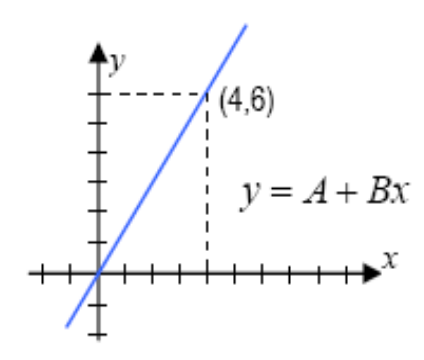
\includegraphics[width=0.35\textwidth]{images/reta01}
	\caption{Exemplo 01}
\end{figure}

1. Limpar a memória: \keystroke{$f$} \keystroke{$\sum$}

2. Entrar com os valores: \keystroke{$0$} \keystroke{$Enter$} \keystroke{$0$} \keystroke{$\sum+$} \keystroke{$6$} \keystroke{$Enter$} \keystroke{$4$} \keystroke{$\sum+$}

3. Calcular a inclinação: \keystroke{$1$} \keystroke{$g$} \keystroke{$\hat{y},r$}

4. Calcular o valor da ordenada: \keystroke{$8$} \keystroke{$g$} \keystroke{$\hat{y},r$} 

E assim temos uma inclinação de \textbf{1,50} e para abcissa com valor 8 a ordenada é igual a \textbf{12}.

\textbf{Problema 2}: Calcular o ponto de interceptação-y, a inclinação para caracterizar a linha reta e o valor da abcissa quando a ordenada for igual a 5 com base na informação do seguinte gráfico:
\begin{figure}[H]
	\centering
	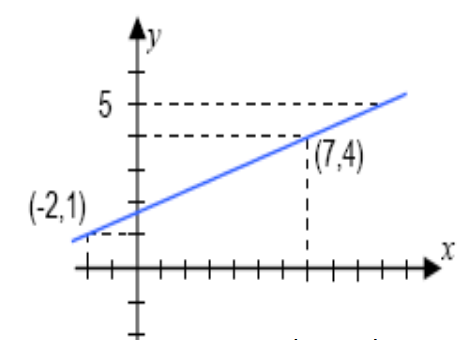
\includegraphics[width=0.35\textwidth]{images/reta02}
	\caption{Exemplo 02}
\end{figure}

1. Limpar a memória: \\
\keystroke{$f$} \keystroke{$\sum$}

2. Entrar com os valores: \\
\keystroke{$1$} \keystroke{$Enter$} \keystroke{$2$} \keystroke{$CHS$} \keystroke{$\sum+$} \keystroke{$4$} \keystroke{$Enter$} \keystroke{$7$} \keystroke{$\sum+$}

3. Calcular a interceptação-y (A): 1,67 \\
\keystroke{$0$} \keystroke{$g$} \keystroke{$\hat{y},r$}

4. Calcular a inclinação (B): 0,33 \\
\keystroke{$1$} \keystroke{$g$} \keystroke{$\hat{y},r$} \keystroke{$x \lessgtr y$} \keystroke{$R \downarrow$} \keystroke{$x \lessgtr y$} \keystroke{$-$}

5. Calcular o valor da abcissa: 10 \\
\keystroke{$5$} \keystroke{$g$} \keystroke{$\hat{x},r$} 

\textbf{Problema 3}: Estimar as vendas previstas de uma fábrica para o ano de 2019 e em que ano as vendas chegam a 130.000 unidades conforme o seguinte detalhamento (as vendas estão em mil unidades): 2010 - 58; 2011 - 66; 2012 - 72; 2013 - 77; 2014 - 81; 2015 - 85.

Uma forma de estimar o comportamento das vendas futuras consiste em aplicar o Método dos Mínimos Quadrados, que permite encontrar a melhor reta que se ajusta aos pontos.

1. Limpar a memória: \\
\keystroke{$f$} \keystroke{$\sum$}

2. Entrar com os valores (para agilizar a digitação podemos usar o ano com 2 dígitos): \\
\keystroke{$5$} \keystroke{$8$} \keystroke{$Enter$} \keystroke{$1$} \keystroke{$0$} \keystroke{$\sum+$} \\
\keystroke{$6$} \keystroke{$6$} \keystroke{$Enter$} \keystroke{$1$} \keystroke{$1$} \keystroke{$\sum+$} \\
\keystroke{$7$} \keystroke{$2$} \keystroke{$Enter$} \keystroke{$1$} \keystroke{$2$} \keystroke{$\sum+$} \\
\keystroke{$7$} \keystroke{$7$} \keystroke{$Enter$} \keystroke{$1$} \keystroke{$3$} \keystroke{$\sum+$} \\
\keystroke{$8$} \keystroke{$1$} \keystroke{$Enter$} \keystroke{$1$} \keystroke{$4$} \keystroke{$\sum+$} \\
\keystroke{$8$} \keystroke{$5$} \keystroke{$Enter$} \keystroke{$1$} \keystroke{$5$} \keystroke{$\sum+$} 

3. Vendas previstas para o ano de 2019: 107,52 mil unidades \\ 
\keystroke{$1$} \keystroke{$9$} \keystroke{$g$} \keystroke{$\hat{y},r$}

4. Ano para 130.000 unidades: 2023 \\
\keystroke{$1$} \keystroke{$3$} \keystroke{$0$} \keystroke{$g$} \keystroke{$\hat{x},r$}

\subsection*{Programação com Permutação e Combinação}
Programar na HP-12C consiste em gravar uma sequência de teclas, este é um recurso muito útil para determinadas situações. É possível inserir no máximo 99 linhas na memória. As principais teclas a saber são: \vspace{-1em}
\begin{itemize}
	\item \keystroke{$R/S$} \textit{RUN/STOP}, iniciar ou interromper a execução de um programa
	\item \keystroke{$f$} \keystroke{$P/R$} \textit{PROGRAM/RUN}, colocar a calculadora em modo de programação ou execução
	\item \keystroke{$g$} \keystroke{$PSE$} \textit{PAUSE}, fornecer uma pausa com cerca de 1 seg. na execução do programa
	\item \keystroke{$f$} \keystroke{$PRGM$} \textit{CLEAR PROGRAMS}, limpar os programas registrados na memória da calculadora
	\item \keystroke{$g$} \keystroke{$GTO$} \textit{GO TO}, executar um desvio de rotina no programa
	\item \keystroke{$g$} \keystroke{$BST$} \textit{STEP}, executar o programa passo a passo
\end{itemize}

\textbf{Permutação} (também chamada de Arranjo Simples) é um subconjunto ordenado em um conjunto de objetos distintos. O número de permutações possíveis, cada uma contendo n objetos, que podem ser formadas a partir de m objetos distintos é dado por: $_mP_n = m! \div (m - n)!$ Lembre-se que na permutação não existe repetição e o número de elementos a serem tomados para compor o resultado deve ser igual ao número de elementos no conjunto.

Por exemplo, seja T um conjunto com elementos: \{A,B,C,D\}, e queremos realizar agrupamentos com 2 elementos quantos arranjos podemos obter. Para resolvermos na calculadora criamos o seguinte programa:

\keystroke{$f$} \keystroke{$P/R$} \\
\keystroke{$f$} \keystroke{$PRGM$} - 00 \\
\keystroke{$STO$} \keystroke{$0$} - 01 \\
\keystroke{$x \lessgtr y$} - 02 \\
\keystroke{$g$} \keystroke{$n!$} - 03 \\
\keystroke{$g$} \keystroke{$LST x$} - 04 \\
\keystroke{$RCL$} \keystroke{$0$} - 05 \\
\keystroke{$-$} - 06 \\
\keystroke{$g$} \keystroke{$n!$} - 07 \\
\keystroke{$\div$} - 08 \\
\keystroke{$g$} \keystroke{$GTO$} \keystroke{$0$} \keystroke{$0$} - 09 \\
\keystroke{$f$} \keystroke{$P/R$}

E para executar o programa: \keystroke{$4$} \keystroke{$Enter$} \keystroke{$2$} \keystroke{$R/S$} e temos como resposta 12. Ou seja: \\
$_4P_2$ = \{AB, AC, AD, BA, BC, BD, CA, CB, CD, DA, DB, DC\}

\textbf{Problema 1}: De quantas maneiras diferentes 10 pessoas podem sentar em um banco se só existem 4 lugares disponíveis? ($_{10}P_4$)

\keystroke{$1$} \keystroke{$0$} \keystroke{$Enter$} \keystroke{$4$} \keystroke{$R/S$}

E temos 5.040 maneiras diferentes.

\textbf{Problema 2}: Uma corrida com 20 atletas vai premiar os 5 primeiros, quantos arranjos são possíveis realizar? ($_{20}P_5$)

\keystroke{$2$} \keystroke{$0$} \keystroke{$Enter$} \keystroke{$5$} \keystroke{$R/S$}

E temos 1.860.480 maneiras diferentes.

\textbf{Combinação} é uma seleção com um ou mais conjuntos de objetos distintos, independentemente da ordem. O número de combinações possíveis, cada uma contendo n objetos, que podem ser formadas a partir de uma coleção de m objetos distintos é dado por: $_mC_n = m! \div (m - n)!n!$

Por exemplo, seja T um conjunto com elementos: \{A,B,C,D\}, e queremos realizar agrupamentos com 2 elementos quantos arranjos podemos obter sem a repetição desses. Para resolvermos na calculadora criamos o seguinte programa:

\keystroke{$f$} \keystroke{$P/R$} \\
\keystroke{$f$} \keystroke{$PRGM$} - 00 \\
\keystroke{$STO$} \keystroke{$0$} - 01 \\
\keystroke{$x \lessgtr y$} - 02 \\
\keystroke{$g$} \keystroke{$n!$} - 03 \\
\keystroke{$g$} \keystroke{$LST x$} - 04 \\
\keystroke{$RCL$} \keystroke{$0$} - 05 \\
\keystroke{$-$} - 06 \\
\keystroke{$g$} \keystroke{$n!$} - 07 \\
\keystroke{$RCL$} \keystroke{$0$} - 08 \\
\keystroke{$g$} \keystroke{$n!$} - 09 \\
\keystroke{$\times$} - 10 \\
\keystroke{$\div$} - 11 \\
\keystroke{$g$} \keystroke{$GTO$} \keystroke{$0$} \keystroke{$0$} - 12 \\
\keystroke{$f$} \keystroke{$P/R$}

E para executar o programa: \keystroke{$4$} \keystroke{$Enter$} \keystroke{$2$} \keystroke{$R/S$} e temos como resposta 6. Ou seja: \\
$_4C_2$ = \{AB ou BA, AC ou CA, AD ou DA, BC ou CB, BD ou DB, CD ou DC\}

\textbf{Problema 1}: Um coordenador precisa selecionar um comitê formado por três pessoas entre os sete engenheiros que trabalham para ele. De quantas maneiras diferentes o comitê pode ser selecionado? $_7C_3$

\keystroke{$7$} \keystroke{$Enter$} \keystroke{$3$} \keystroke{$R/S$}

E temos 35 maneiras diferentes.

\textbf{Problema 2}: A megassena consiste em uma cartela de 60 números dentre os quais devemos acertar 6 para ganharmos o prêmio principal, quantas possibilidades existem? $_60C_6$

\keystroke{$6$} \keystroke{$0$} \keystroke{$Enter$} \keystroke{$6$} \keystroke{$R/S$}

E temos 50.063.860 maneiras diferentes.






\section*{Conclusão}
O mais interessante que para praticar todos os conceitos que vimos nesta apostila não é necessário possuir uma HP12C e além do software indicado ainda é possível encontrá-la em vários sites \cite{online} que apresentam versões online da mesma tornando possível testar todas as suas funcionalidades antes de adquiri-la.

Sou um entusiasta do mundo \textbf{Open Source} e novas tecnologias. Qual a diferença entre Livre e Open Source? \underline{Livre} significa que esta apostila é gratuita e pode ser compartilhada a vontade. \underline{Open Source} além de livre todos os arquivos que permitem a geração desta (chamados de arquivos fontes) devem ser disponibilizados para que qualquer pessoa possa modificar ao seu prazer, gerar novas, complementar ou fazer o que quiser. Os fontes da apostila (que foi produzida com o LaTex) está disponibilizado no GitHub \cite{github}. Veja ainda outros artigos que publico sobre tecnologia através do meu Blog Oficial \cite{fernandoanselmo}.

%--------------------------------------------------------------------------
% REFERÊNCIAS
%--------------------------------------------------------------------------
\begin{thebibliography}{4}
	\bibitem{hp12c} 
	Versão HP12C Platinum \\
	\url{https://sourceforge.net/projects/finanx/}
	
	\bibitem{online} 
	Versão OnLine \\
	\url{https://www.fazerfacil.com.br/calculadoras/hp12c.html}
	
		\bibitem{fernandoanselmo} 
	Fernando Anselmo - Blog Oficial de Tecnologia \\
	\url{http://www.fernandoanselmo.blogspot.com.br/}
	
	\bibitem{publicacao} 
	Encontre essa e outras publicações em \\
	\url{https://cetrex.academia.edu/FernandoAnselmo}
	
	\bibitem{github} 
	Repositório para os fontes da apostila \\
	\url{https://github.com/fernandoans/publicacoes}
\end{thebibliography}

\newpage
\begin{figure}[H]
	\centering
	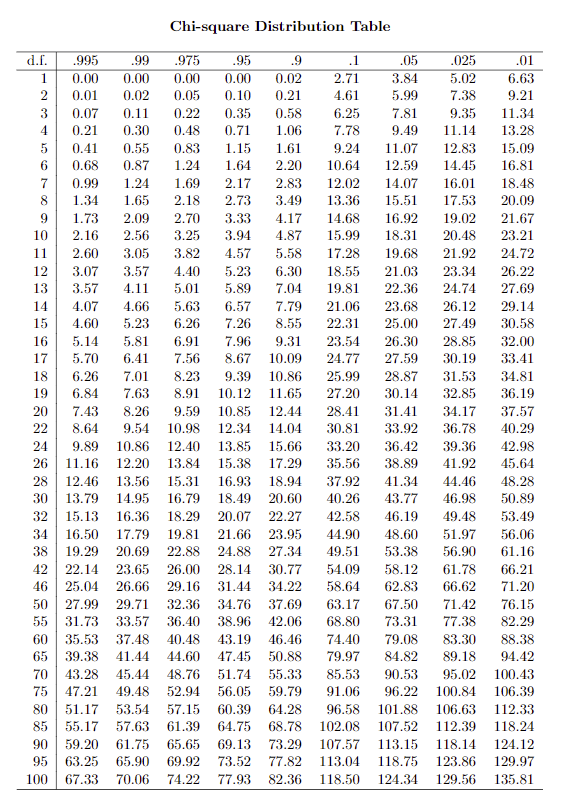
\includegraphics[width=1.0\textwidth]{images/tabela-chi-square}
	\caption{Tabela Qui-quadrado}
\end{figure}

\end{document}

